\documentclass[border=0bp]{standalone}
\usepackage{newtxtext,newtxmath}
\usepackage{tikz,pgfplots}
\pgfplotsset{compat=1.17}
\usetikzlibrary{arrows.meta,calc}
\definecolor{teal}{HTML}{167C80}
\definecolor{orange}{HTML}{D55E00}
\definecolor{ours}{HTML}{0072B2}
\definecolor{blue}{HTML}{0072B2}
\definecolor{lag}{HTML}{A0467E}
\definecolor{gray}{HTML}{59636A}
\definecolor{ink}{HTML}{23343B}
\definecolor{hard}{HTML}{C43C39}
\definecolor{cost}{HTML}{E69F00}
\newcommand{\bodyfont}{\fontsize{7.5}{8.5}\selectfont}
\newcommand{\ticks}{\fontsize{7}{7.5}\selectfont}
\newcommand{\titlefont}{\fontsize{8.8}{9.6}\selectfont\bfseries}
\newcommand{\mathfont}{\fontsize{8.6}{9.6}\selectfont}
\tikzset{
  every node/.style={font=\bodyfont,text=ink,inner sep=0pt,outer sep=0pt},
  module/.style={rounded corners=3bp,line width=.6bp},
  flow/.style={line width=.8bp,-{Stealth[length=3.5bp,width=3bp]}},
  title/.style={font=\titlefont},
  formula/.style={font=\mathfont},
  chip/.style={rounded corners=2bp,inner xsep=3bp,inner ysep=1.6bp}
}
\begin{document}
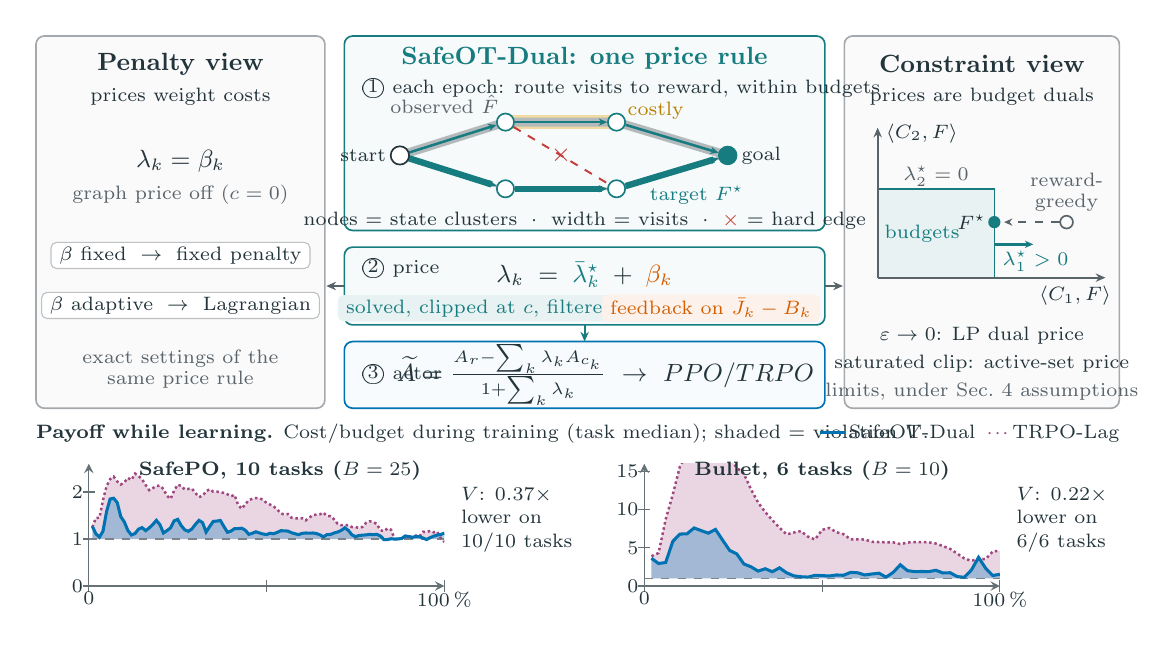
\begin{tikzpicture}[x=1bp,y=-1bp]
\path[use as bounding box] (0,0) rectangle (396,212);

% ---------------- columns (same scaffold as v16) ----------------
\draw[module,draw=gray!55,fill=gray!3] (3,3) rectangle (107,137);
\draw[module,draw=gray!55,fill=gray!3] (294,3) rectangle (393,137);
\draw[module,draw=teal,fill=teal!4] (114,3) rectangle (287,73);
\draw[module,draw=teal,fill=teal!4] (114,79) rectangle (287,107);
\draw[module,draw=blue,fill=blue!3] (114,113) rectangle (287,137);

% ---------------- center (1): the budgeted flow, drawn as re-routing ----------------
\node[title,text=teal] at (200.5,11) {SafeOT-Dual: one price rule};
\node[anchor=west] at (120,22) {\textcircled{\scriptsize 1} each epoch: route visits to reward, within budgets};
\coordinate (s) at (134,46); \coordinate (a) at (172,34); \coordinate (b) at (212,34);
\coordinate (c) at (172,58); \coordinate (d) at (212,58); \coordinate (g) at (252,46);
% costly edge highlighted
\draw[cost,line width=5bp,line cap=round,opacity=.35] (a) -- (b);
% observed flow F-hat (faint gray underlay): mostly the short costly route
\draw[gray!45,line width=3.2bp,line cap=round] (s) -- (a) -- (b) -- (g);
\draw[gray!45,line width=1bp,line cap=round] (s) -- (c) -- (d) -- (g);
% projected flow F-star: the costly route is thinned, the detour carries the flow
\begin{scope}[teal,-{Stealth[length=3bp,width=2.6bp]},shorten >=3.4bp,shorten <=3.4bp]
\draw[line width=.9bp] (s) -- (a); \draw[line width=.9bp] (a) -- (b); \draw[line width=.9bp] (b) -- (g);
\draw[line width=2.3bp] (s) -- (c); \draw[line width=2.3bp] (c) -- (d); \draw[line width=2.3bp] (d) -- (g);
\end{scope}
\draw[hard,dashed,line width=.7bp,shorten >=3.4bp,shorten <=3.4bp] (a) -- (d);
\node[text=hard,font=\fontsize{9}{9}\selectfont] at (192,46) {$\times$};
\foreach \n in {a,b,c,d} \filldraw[fill=white,draw=teal,line width=.6bp] (\n) circle (3.1bp);
\filldraw[fill=white,draw=ink,line width=.6bp] (s) circle (3.3bp);
\filldraw[fill=teal,draw=teal] (g) circle (3.3bp);
\node[anchor=east] at (129,46) {start};
\node[anchor=west] at (257,46) {goal};
\node[anchor=west,text=cost!80!black,font=\ticks] at (216,30) {costly};
\node[anchor=south,font=\ticks,align=center] at (200.5,72.6) {nodes $=$ state clusters \;$\cdot$\; width $=$ visits \;$\cdot$\; {\color{hard}$\times$} $=$ hard edge};
\node[anchor=south,font=\ticks,text=gray] at (150,31) {observed $\hat F$};
\node[anchor=north west,font=\ticks,text=teal] at (224,57) {target $F^\star$};

% ---------------- center (2): price ----------------
\node[anchor=west] at (120,87) {\textcircled{\scriptsize 2} price};
\node[formula] at (200.5,89) {$\lambda_k \;=\; {\color{teal}\bar\lambda^\star_k} \;+\; {\color{orange}\beta_k}$};
\node[chip,text=teal,fill=teal!10] at (163,101) {solved, clipped at $c$, filtered};
\node[chip,text=orange,fill=orange!8] at (246,101) {feedback on $\bar J_k-B_k$};
\draw[flow,teal] (200.5,107) -- (200.5,113);

% ---------------- center (3): actor ----------------
\node[anchor=west] at (120,125) {\textcircled{\scriptsize 3} actor};
\node[formula] at (208,125) {$\widetilde A=\frac{A_r-\sum_k\lambda_k A_{c_k}}{1+\sum_k\lambda_k}\ \to\ \text{PPO/TRPO}$};

% ---------------- left: penalty view (exact settings) ----------------
\node[title] at (55,13) {Penalty view};
\node at (55,25) {prices weight costs};
\node[formula] at (55,48) {$\lambda_k=\beta_k$};
\node[text=gray] at (55,60) {graph price off ($c=0$)};
\node[chip,fill=white,draw=gray!40] at (55,82) {$\beta$ fixed $\;\to\;$ fixed penalty};
\node[chip,fill=white,draw=gray!40] at (55,100) {$\beta$ adaptive $\;\to\;$ Lagrangian};
\draw[flow,gray] (114,93) -- (107.5,93);
\node[text=gray,font=\ticks,align=center] at (55,123) {exact settings of the\\ same price rule};

% ---------------- right: constraint view (conditional limits) ----------------
\node[title] at (343.5,13) {Constraint view};
\node at (343.5,25) {prices are budget duals};
\fill[teal!10] (306,90) rectangle (348,58);
\draw[teal,line width=.6bp] (306,58) -- (348,58) -- (348,90);
\draw[flow,gray,line width=.6bp] (306,90) -- (388,90);
\draw[flow,gray,line width=.6bp] (306,90) -- (306,36);
\node[anchor=west,font=\ticks] at (309,38) {$\langle C_2,F\rangle$};
\node[anchor=north east,font=\ticks] at (390,93) {$\langle C_1,F\rangle$};
\node[font=\ticks,text=teal] at (322,74) {budgets};
% reward-greedy point outside, projected onto the binding face
\draw[gray,line width=.6bp] (374,70) circle (2.3bp);
\node[anchor=south,font=\ticks,text=gray,align=center] at (374,66) {reward-\\greedy};
\draw[-{Stealth[length=3bp,width=2.6bp]},gray,line width=.6bp,dashed] (371.5,70) -- (351.5,70);
\fill[teal] (348,70) circle (2.2bp);
\node[anchor=east,font=\ticks] at (345,70) {$F^\star$};
\draw[-{Stealth[length=3bp,width=2.6bp]},orange!0!teal,line width=.9bp] (348,78) -- (362,78);
\node[anchor=west,font=\ticks,text=teal] at (351,84) {$\lambda^\star_1>0$};
\node[anchor=south,font=\ticks,text=gray] at (327,57) {$\lambda^\star_2=0$};
\draw[flow,gray] (287,93) -- (293.5,93);
\node[font=\ticks,align=center] at (343.5,111) {$\varepsilon\to0$: LP dual price};
\node[font=\ticks,align=center] at (343.5,121) {saturated clip: active-set price};
\node[font=\ticks,text=gray] at (343.5,131) {limits, under Sec.~4 assumptions};

% ---------------- bottom strip: what the solved price buys (real data) ----------------
\node[anchor=west,font=\bodyfont] at (3,146) {\textbf{Payoff while learning.} Cost$/$budget during training (task median); shaded $=$ violation $V$.};
\node[anchor=east,font=\ticks] at (393,146) {{\color{ours}\rule[1.6bp]{9bp}{1.1bp}}\,SafeOT-Dual\enspace{\color{lag}$\cdot\!\cdot\!\cdot$}\,TRPO-Lag};

\begin{axis}[at={(22bp,-201bp)},anchor=south west,width=128bp,height=44bp,scale only axis,
  xmin=0,xmax=100,ymin=0,ymax=2.6,xtick={0,50,100},ytick={0,1,2},
  axis lines=left,axis line style={ink!70,line width=.5bp},tick style={ink!70,line width=.4bp},
  tick label style={font=\ticks},label style={font=\ticks},
  xticklabels={0,,100\,\%},
  clip=true]
\addplot[draw=none,fill=lag,fill opacity=.22] coordinates {(1,1.251) (2,1.448) (3,1.451) (4,1.831) (5,2.121) (6,2.273) (7,2.327) (8,2.223) (9,2.158) (10,2.205) (11,2.299) (12,2.256) (13,2.392) (14,2.338) (15,2.268) (16,2.148) (17,2.038) (18,2.082) (19,2.127) (20,2.136) (21,2.062) (22,1.918) (23,1.854) (24,2.029) (25,2.155) (26,2.129) (27,2.052) (28,2.067) (29,2.073) (30,1.977) (31,1.893) (32,1.917) (33,2.016) (34,2.058) (35,2.007) (36,2.008) (37,1.992) (38,1.982) (39,1.951) (40,1.910) (41,1.936) (42,1.723) (43,1.644) (44,1.738) (45,1.825) (46,1.856) (47,1.871) (48,1.866) (49,1.834) (50,1.766) (51,1.732) (52,1.693) (53,1.628) (54,1.546) (55,1.520) (56,1.532) (57,1.453) (58,1.441) (59,1.435) (60,1.442) (61,1.396) (62,1.455) (63,1.506) (64,1.519) (65,1.525) (66,1.561) (67,1.490) (68,1.486) (69,1.418) (70,1.323) (71,1.293) (72,1.298) (73,1.291) (74,1.255) (75,1.253) (76,1.237) (77,1.257) (78,1.346) (79,1.378) (80,1.360) (81,1.321) (82,1.190) (83,1.162) (84,1.225) (85,1.198) (86,1.002) (87,1.000) (88,1.015) (89,1.038) (90,1.051) (91,1.044) (92,1.073) (93,1.055) (94,1.154) (95,1.144) (96,1.175) (97,1.142) (98,1.155) (99,1.017) (100,1.000) (100,1.000) (1,1.000)} -- cycle;
\addplot[draw=none,fill=ours,fill opacity=.30] coordinates {(1,1.269) (2,1.111) (3,1.039) (4,1.168) (5,1.583) (6,1.851) (7,1.867) (8,1.774) (9,1.476) (10,1.362) (11,1.180) (12,1.085) (13,1.117) (14,1.211) (15,1.242) (16,1.178) (17,1.236) (18,1.309) (19,1.396) (20,1.307) (21,1.128) (22,1.179) (23,1.237) (24,1.386) (25,1.418) (26,1.285) (27,1.195) (28,1.164) (29,1.213) (30,1.313) (31,1.396) (32,1.348) (33,1.147) (34,1.265) (35,1.374) (36,1.381) (37,1.395) (38,1.265) (39,1.143) (40,1.169) (41,1.221) (42,1.219) (43,1.230) (44,1.189) (45,1.099) (46,1.122) (47,1.153) (48,1.128) (49,1.106) (50,1.095) (51,1.122) (52,1.112) (53,1.141) (54,1.176) (55,1.174) (56,1.168) (57,1.134) (58,1.112) (59,1.092) (60,1.120) (61,1.128) (62,1.124) (63,1.128) (64,1.117) (65,1.089) (66,1.045) (67,1.094) (68,1.097) (69,1.128) (70,1.149) (71,1.182) (72,1.237) (73,1.183) (74,1.089) (75,1.049) (76,1.075) (77,1.082) (78,1.087) (79,1.099) (80,1.092) (81,1.100) (82,1.064) (83,1.000) (84,1.000) (85,1.006) (86,1.000) (87,1.001) (88,1.011) (89,1.065) (90,1.052) (91,1.036) (92,1.055) (93,1.050) (94,1.021) (95,1.000) (96,1.028) (97,1.061) (98,1.084) (99,1.096) (100,1.125) (100,1.000) (1,1.000)} -- cycle;
\addplot[ink!60,dashed,line width=.5bp] coordinates {(0,1) (100,1)};
\addplot[lag,line width=.9bp,densely dotted] coordinates {(1,1.251) (2,1.448) (3,1.451) (4,1.831) (5,2.121) (6,2.273) (7,2.327) (8,2.223) (9,2.158) (10,2.205) (11,2.299) (12,2.256) (13,2.392) (14,2.338) (15,2.268) (16,2.148) (17,2.038) (18,2.082) (19,2.127) (20,2.136) (21,2.062) (22,1.918) (23,1.854) (24,2.029) (25,2.155) (26,2.129) (27,2.052) (28,2.067) (29,2.073) (30,1.977) (31,1.893) (32,1.917) (33,2.016) (34,2.058) (35,2.007) (36,2.008) (37,1.992) (38,1.982) (39,1.951) (40,1.910) (41,1.936) (42,1.723) (43,1.644) (44,1.738) (45,1.825) (46,1.856) (47,1.871) (48,1.866) (49,1.834) (50,1.766) (51,1.732) (52,1.693) (53,1.628) (54,1.546) (55,1.520) (56,1.532) (57,1.453) (58,1.441) (59,1.435) (60,1.442) (61,1.396) (62,1.455) (63,1.506) (64,1.519) (65,1.525) (66,1.561) (67,1.490) (68,1.486) (69,1.418) (70,1.323) (71,1.293) (72,1.298) (73,1.291) (74,1.255) (75,1.253) (76,1.237) (77,1.257) (78,1.346) (79,1.378) (80,1.360) (81,1.321) (82,1.190) (83,1.162) (84,1.225) (85,1.198) (86,1.002) (87,0.999) (88,1.015) (89,1.038) (90,1.051) (91,1.044) (92,1.073) (93,1.055) (94,1.154) (95,1.144) (96,1.175) (97,1.142) (98,1.155) (99,1.017) (100,0.935)};
\addplot[ours,line width=1.1bp] coordinates {(1,1.269) (2,1.111) (3,1.039) (4,1.168) (5,1.583) (6,1.851) (7,1.867) (8,1.774) (9,1.476) (10,1.362) (11,1.180) (12,1.085) (13,1.117) (14,1.211) (15,1.242) (16,1.178) (17,1.236) (18,1.309) (19,1.396) (20,1.307) (21,1.128) (22,1.179) (23,1.237) (24,1.386) (25,1.418) (26,1.285) (27,1.195) (28,1.164) (29,1.213) (30,1.313) (31,1.396) (32,1.348) (33,1.147) (34,1.265) (35,1.374) (36,1.381) (37,1.395) (38,1.265) (39,1.143) (40,1.169) (41,1.221) (42,1.219) (43,1.230) (44,1.189) (45,1.099) (46,1.122) (47,1.153) (48,1.128) (49,1.106) (50,1.095) (51,1.122) (52,1.112) (53,1.141) (54,1.176) (55,1.174) (56,1.168) (57,1.134) (58,1.112) (59,1.092) (60,1.120) (61,1.128) (62,1.124) (63,1.128) (64,1.117) (65,1.089) (66,1.045) (67,1.094) (68,1.097) (69,1.128) (70,1.149) (71,1.182) (72,1.237) (73,1.183) (74,1.089) (75,1.049) (76,1.075) (77,1.082) (78,1.087) (79,1.099) (80,1.092) (81,1.100) (82,1.064) (83,0.988) (84,0.988) (85,1.006) (86,0.998) (87,1.001) (88,1.011) (89,1.065) (90,1.052) (91,1.036) (92,1.055) (93,1.050) (94,1.021) (95,0.989) (96,1.028) (97,1.061) (98,1.084) (99,1.096) (100,1.125)};
\end{axis}
\node[anchor=north west,font=\bodyfont\bfseries] at (40bp,-156bp) {SafePO, 10 tasks ($B=25$)};

\node[anchor=west,align=left,font=\bodyfont] at (156bp,-177bp) {$V$: $0.37\times$\\lower on\\10/10 tasks};

\begin{axis}[at={(222bp,-201bp)},anchor=south west,width=128bp,height=44bp,scale only axis,
  xmin=0,xmax=100,ymin=0,ymax=16,xtick={0,50,100},ytick={0,5,10,15},
  axis lines=left,axis line style={ink!70,line width=.5bp},tick style={ink!70,line width=.4bp},
  tick label style={font=\ticks},label style={font=\ticks},
  xticklabels={0,,100\,\%},
  clip=true]
\addplot[draw=none,fill=lag,fill opacity=.22] coordinates {(2,3.908) (4,4.317) (6,8.715) (8,11.962) (10,15.658) (12,17.248) (14,18.251) (16,19.731) (18,20.049) (20,19.471) (22,17.870) (24,16.785) (26,15.480) (28,14.687) (30,12.662) (32,10.923) (34,9.677) (36,8.621) (38,7.641) (40,6.750) (42,6.994) (44,7.185) (46,6.472) (48,6.087) (50,7.349) (52,7.594) (54,7.054) (56,6.788) (58,6.117) (60,6.105) (62,6.083) (64,5.791) (66,5.754) (68,5.715) (70,5.712) (72,5.485) (74,5.683) (76,5.758) (78,5.748) (80,5.717) (82,5.561) (84,5.221) (86,4.859) (88,4.239) (90,3.602) (92,3.297) (94,3.564) (96,3.516) (98,4.529) (100,4.603) (100,1.000) (2,1.000)} -- cycle;
\addplot[draw=none,fill=ours,fill opacity=.30] coordinates {(2,3.630) (4,2.946) (6,3.078) (8,5.842) (10,6.799) (12,6.833) (14,7.597) (16,7.246) (18,6.918) (20,7.407) (22,6.014) (24,4.658) (26,4.200) (28,2.880) (30,2.514) (32,1.953) (34,2.260) (36,1.869) (38,2.377) (40,1.736) (42,1.339) (44,1.212) (46,1.167) (48,1.395) (50,1.357) (52,1.313) (54,1.446) (56,1.403) (58,1.781) (60,1.732) (62,1.445) (64,1.573) (66,1.675) (68,1.160) (70,1.790) (72,2.776) (74,2.012) (76,1.883) (78,1.901) (80,1.885) (82,2.057) (84,1.705) (86,1.738) (88,1.234) (90,1.141) (92,2.106) (94,3.746) (96,2.316) (98,1.371) (100,1.539) (100,1.000) (2,1.000)} -- cycle;
\addplot[ink!60,dashed,line width=.5bp] coordinates {(0,1) (100,1)};
\addplot[lag,line width=.9bp,densely dotted] coordinates {(2,3.908) (4,4.317) (6,8.715) (8,11.962) (10,15.658) (12,17.248) (14,18.251) (16,19.731) (18,20.049) (20,19.471) (22,17.870) (24,16.785) (26,15.480) (28,14.687) (30,12.662) (32,10.923) (34,9.677) (36,8.621) (38,7.641) (40,6.750) (42,6.994) (44,7.185) (46,6.472) (48,6.087) (50,7.349) (52,7.594) (54,7.054) (56,6.788) (58,6.117) (60,6.105) (62,6.083) (64,5.791) (66,5.754) (68,5.715) (70,5.712) (72,5.485) (74,5.683) (76,5.758) (78,5.748) (80,5.717) (82,5.561) (84,5.221) (86,4.859) (88,4.239) (90,3.602) (92,3.297) (94,3.564) (96,3.516) (98,4.529) (100,4.603)};
\addplot[ours,line width=1.1bp] coordinates {(2,3.630) (4,2.946) (6,3.078) (8,5.842) (10,6.799) (12,6.833) (14,7.597) (16,7.246) (18,6.918) (20,7.407) (22,6.014) (24,4.658) (26,4.200) (28,2.880) (30,2.514) (32,1.953) (34,2.260) (36,1.869) (38,2.377) (40,1.736) (42,1.339) (44,1.212) (46,1.167) (48,1.395) (50,1.357) (52,1.313) (54,1.446) (56,1.403) (58,1.781) (60,1.732) (62,1.445) (64,1.573) (66,1.675) (68,1.160) (70,1.790) (72,2.776) (74,2.012) (76,1.883) (78,1.901) (80,1.885) (82,2.057) (84,1.705) (86,1.738) (88,1.234) (90,1.141) (92,2.106) (94,3.746) (96,2.316) (98,1.371) (100,1.539)};
\end{axis}
\node[anchor=north west,font=\bodyfont\bfseries] at (240bp,-156bp) {Bullet, 6 tasks ($B=10$)};

\node[anchor=west,align=left,font=\bodyfont] at (356bp,-177bp) {$V$: $0.22\times$\\lower on\\6/6 tasks};

\end{tikzpicture}
\end{document}
